\section{Задание 2. Преобразование координат и базиса.}

\textbf{Условие.}\\
В линейном пространстве со стандартным базисом $E = \Set{e_1, e_2, e_3}$, где
\[e_1 = (1, 0, 0), e_2 = (0, 1, 0), e_3 = (0, 0, 1),\]
заданы системы векторов $A = \Set{a_1, a_2, a_3}$ и $B = \Set{b_1, b_2, b_3}$.\\
$A = \Set{a_1, a_2, a_3}\\
a_1 = (0.433; 0.808; 0.3995)\\
a_2 = (0.25; -0.5335; 0.808)\\
a_3 = (0.866; -0.25; -0.433)\\
B = \Set{b_1, b_2, b_3}\\
b_1 = (4.0801; 1.1495; -1.741 )\\
b_2 = (0.933; -0.259; 2.0155 )\\
b_3 = (2.2811; 3.5245; -2.0915 )\\
x_B = \begin{pmatrix} -0.4231 \\ 0.8077 \\ 1.3462\end{pmatrix}
$
\begin{enumerate}
    \item Покажите, что каждая система образует базис.
    \item Проверьте каждый из этих базисов на ортогональность и нормированность.
    \item Найдите матрицу перехода $T$ из базиса $A$ в базис $B$.
    \item Вектор $x$ в базисе $B$ имеет координаты $x_B = (x_1^\prime, x_2^\prime, x_3^\prime)^T$.
    Найдите его координаты $x_A$ в базисе $A$.
    \item В базисе $E$ изобразите векторы базиса $A$ и вектор $x$.
\end{enumerate}
\vspace{10mm}
\noindent\textbf{Решение.}\\

\begin{enumerate}
    \item 
        A = $\begin{pmatrix} 0.433 & 0.808 & 0.3995 \\ 0.25 & -0.5335 & 0.808 \\ 0.866 & -0.25 & -0.433\end{pmatrix}$ \quad-\quad Чтобы доказать, что система образует базис, приведем к ступенчатому виду. \\\\
        $\begin{pmatrix} 0.433 & 0.808 & 0.3995 \\ 0.25 & -0.5335 & 0.808 \\ 0.866 & -0.25 & -0.433\end{pmatrix} \quad\sim\quad\ 
        \begin{pmatrix} 0.433 & 0.808 & 0.3995 \\ 0 & -1.010.. & 0.577.. \\ 0.866 & -0.25 & -0.433\end{pmatrix}
        \quad\sim\quad\ 
        \begin{pmatrix} 0.433 & 0.808 & 0.3995 \\ 0 & -1.010.. & 0.577.. \\ 0 & 0 & -2,299..\end{pmatrix}
        $\\
        Так как нет нулевых строк, то A является линейно независимой, является базисом.\\
        
        $B = \begin{pmatrix} 4.0801 & 1.1495 & -1.741 \\ 0.933 & -0.259 & 2.0155 \\ 2.2811 & 3.5245 & -2.0915\end{pmatrix}$ \quad-\quad Проводим действия аналогично с матрицей A.\\
        $\begin{pmatrix} 4.0801 & 1.1495 & -1.741 \\ 0.933 & -0.259 & 2.0155 \\ 2.2811 & 3.5245 & -2.0915\end{pmatrix}
        \quad\sim\quad\
        \begin{pmatrix} 4.0801 & 1.1495 & -1.741 \\ 0 & -0.522.. & 2.414.. \\ 2.2811 & 3.5245 & -2.0915\end{pmatrix}
        \quad\sim\quad\ 
        \begin{pmatrix} 4.0801 & 1.1495 & -1.741 \\ 0 & -0.522.. & 2.414.. \\ 0 & 0 & -17.419..\end{pmatrix}
        $\\
        Так как нет нулевых строк, то B является линейно независимой, является базисом.\\

    \item 
        Чтобы узнать ортогональность матриц перемножим попарно вектора.\\
        \begin{figure}[H]
            \centering
            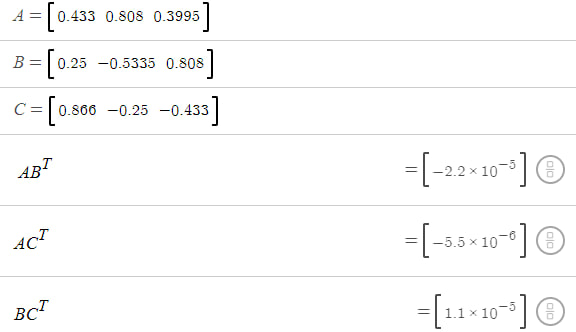
\includegraphics[width=0.6\linewidth]{2_A_orto.png}
            \caption{Матрица A} 
        \end{figure}
        Видно, что погрешность составляет $\sim$10$^{-5}$, что допустимо в нашем случае. A $-$ ортогональна.\\
        \begin{figure}[H]
            \centering
            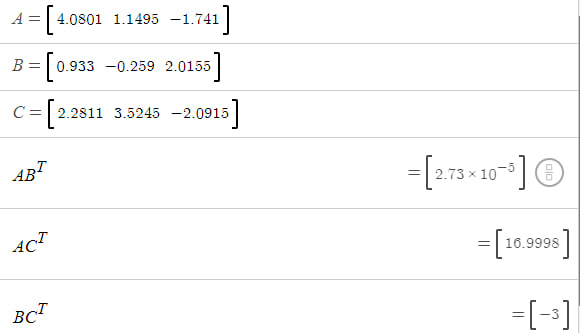
\includegraphics[width=0.6\linewidth]{2_B_orto.png}
            \caption{Матрица B}
        \end{figure}
        Видно, что BC$^T = [-3]$ так что B не ортогональна.\\
        \begin{figure}[H]
            \centering
            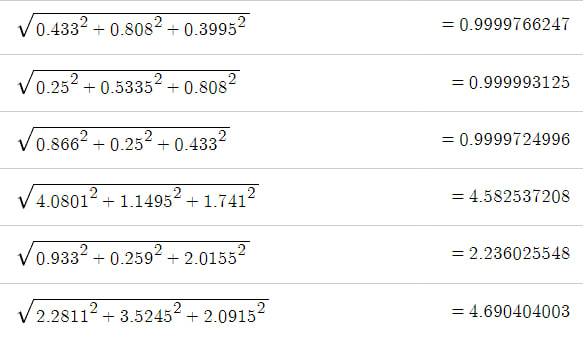
\includegraphics[width=0.6\linewidth]{2_AB_norm.png}
            \caption{Нормы векторов}
        \end{figure}
        Первые три строки $-$ вектора $a_1, a_2, a_3$, а вторые три строки $b_1, b_2, b_3$. Матрица A нормальна, а B нет.\\
        
    \item 
        Матрица перехода T из A в B $-$ это произведение матриц перехода из A в E (A$^{-1}$), и из E в B (B).\\
        \begin{figure}[H]
            \centering
            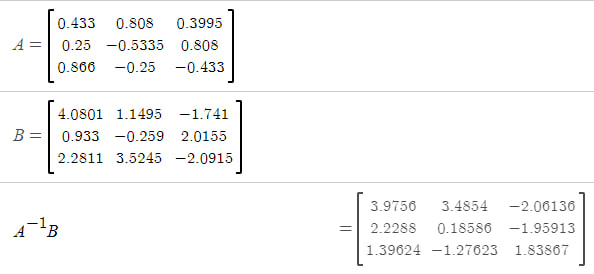
\includegraphics[width=0.6\linewidth]{2_ABT.png}
            \caption{Матрица перехода T}
        \end{figure}

    \item Чтобы найти $x_a$, найдем матрицу перехода B в A и умножим на нее $x_b$.\\
        \begin{figure}[H]
            \centering
            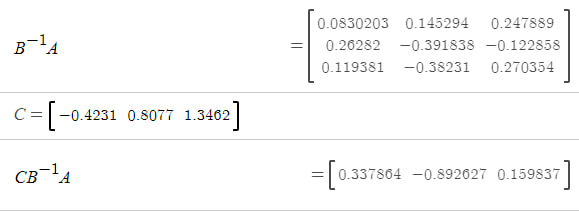
\includegraphics[width=0.6\linewidth]{2_xBAT.png}
            \caption{C $-$ вектор $x_b$}
        \end{figure}

    \item
        Чтобы изобразить вектор $x_b$ перенесем его в базис E, домножив на B$^{-1}$.\\
        \begin{figure}[H]
            \centering
            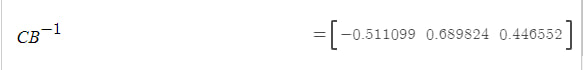
\includegraphics[width=0.6\linewidth]{2_x.png}
            \caption{Вектор x в базисе E}
        \end{figure}
        Далее на рисунке черным изображены базисные вектора A, а красным вектор x.\\
        \begin{figure}[H]
            \centering
            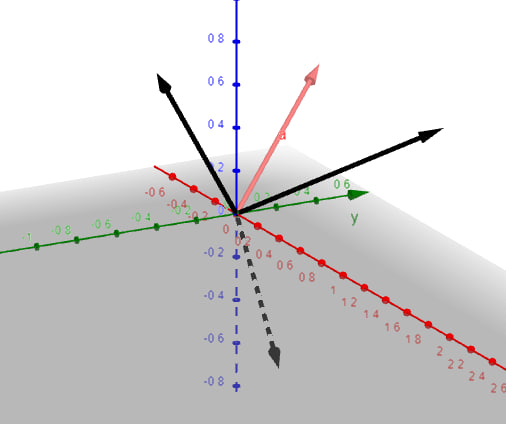
\includegraphics[width=0.6\linewidth]{2_E_graph.png}
            \caption{Вектора в базисе E}
        \end{figure}
\end{enumerate}


\clearpage
